\section{Time reconstruction for charged particles}

Tracks which have been reconstructed using the pixel detector and strip tracker are then propagated to the MTD and spatially matched with compatible clusters.  If a compatible MTD cluster is found, the track parameters are then refit, including this as an additional spatial measurement.  The refitted track is then propagated from the point of closest approach to the beamline, to the MTD front surface, one tracking layer at a time in order to compute the total path length.  This path length is used together with the particle velocity based on the refitted momentum and using the pion mass hypothesis to correct the MTD cluster time back to the point of closest approach to the beamline.  

The efficiency for matching a reconstructed track to an MTD cluster as a function of $p_T$ and $\eta$ is shown in Figure \ref{fig:trackclusterefficiency} for single muon (with 200 average pile-up events and without pile-up) and single pion events in the acceptance region of the the MTD ($|\eta|<3$). Efficiency is flat as a function of $p_{T}$ (above 90\% for muons, around 80\% for pions), and reflects the different geometrical acceptance of the BTL and ETL. Efficiency for pions is also affected by nuclear interactions in the tracker volume as already discussed in section~\ref{sec:btlsim}.

\begin{figure}[!hbtp]
\centering
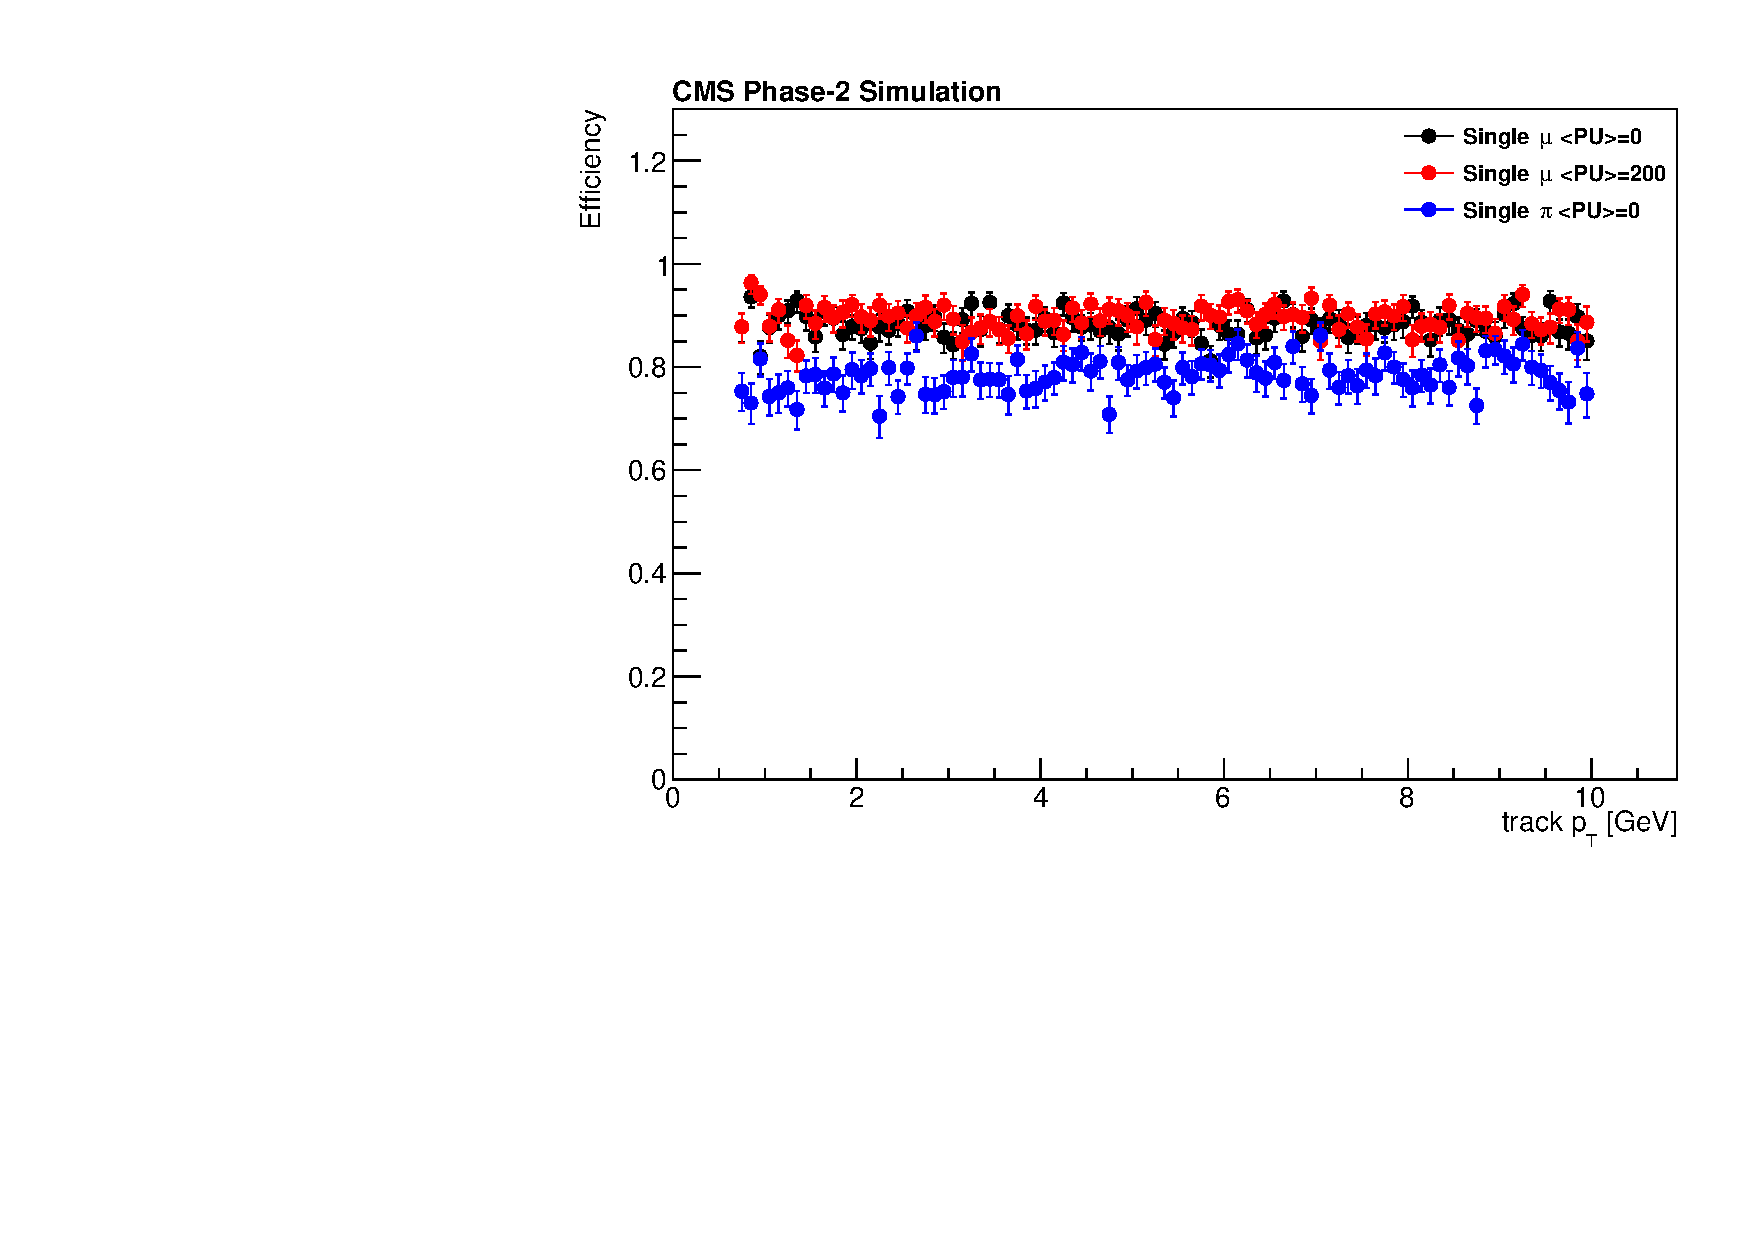
\includegraphics[width=0.48\textwidth]{fig/performance/ClusterAndTracks/divide_mtdTrack_pt_by_track_pt_mupiPUcomp.pdf}
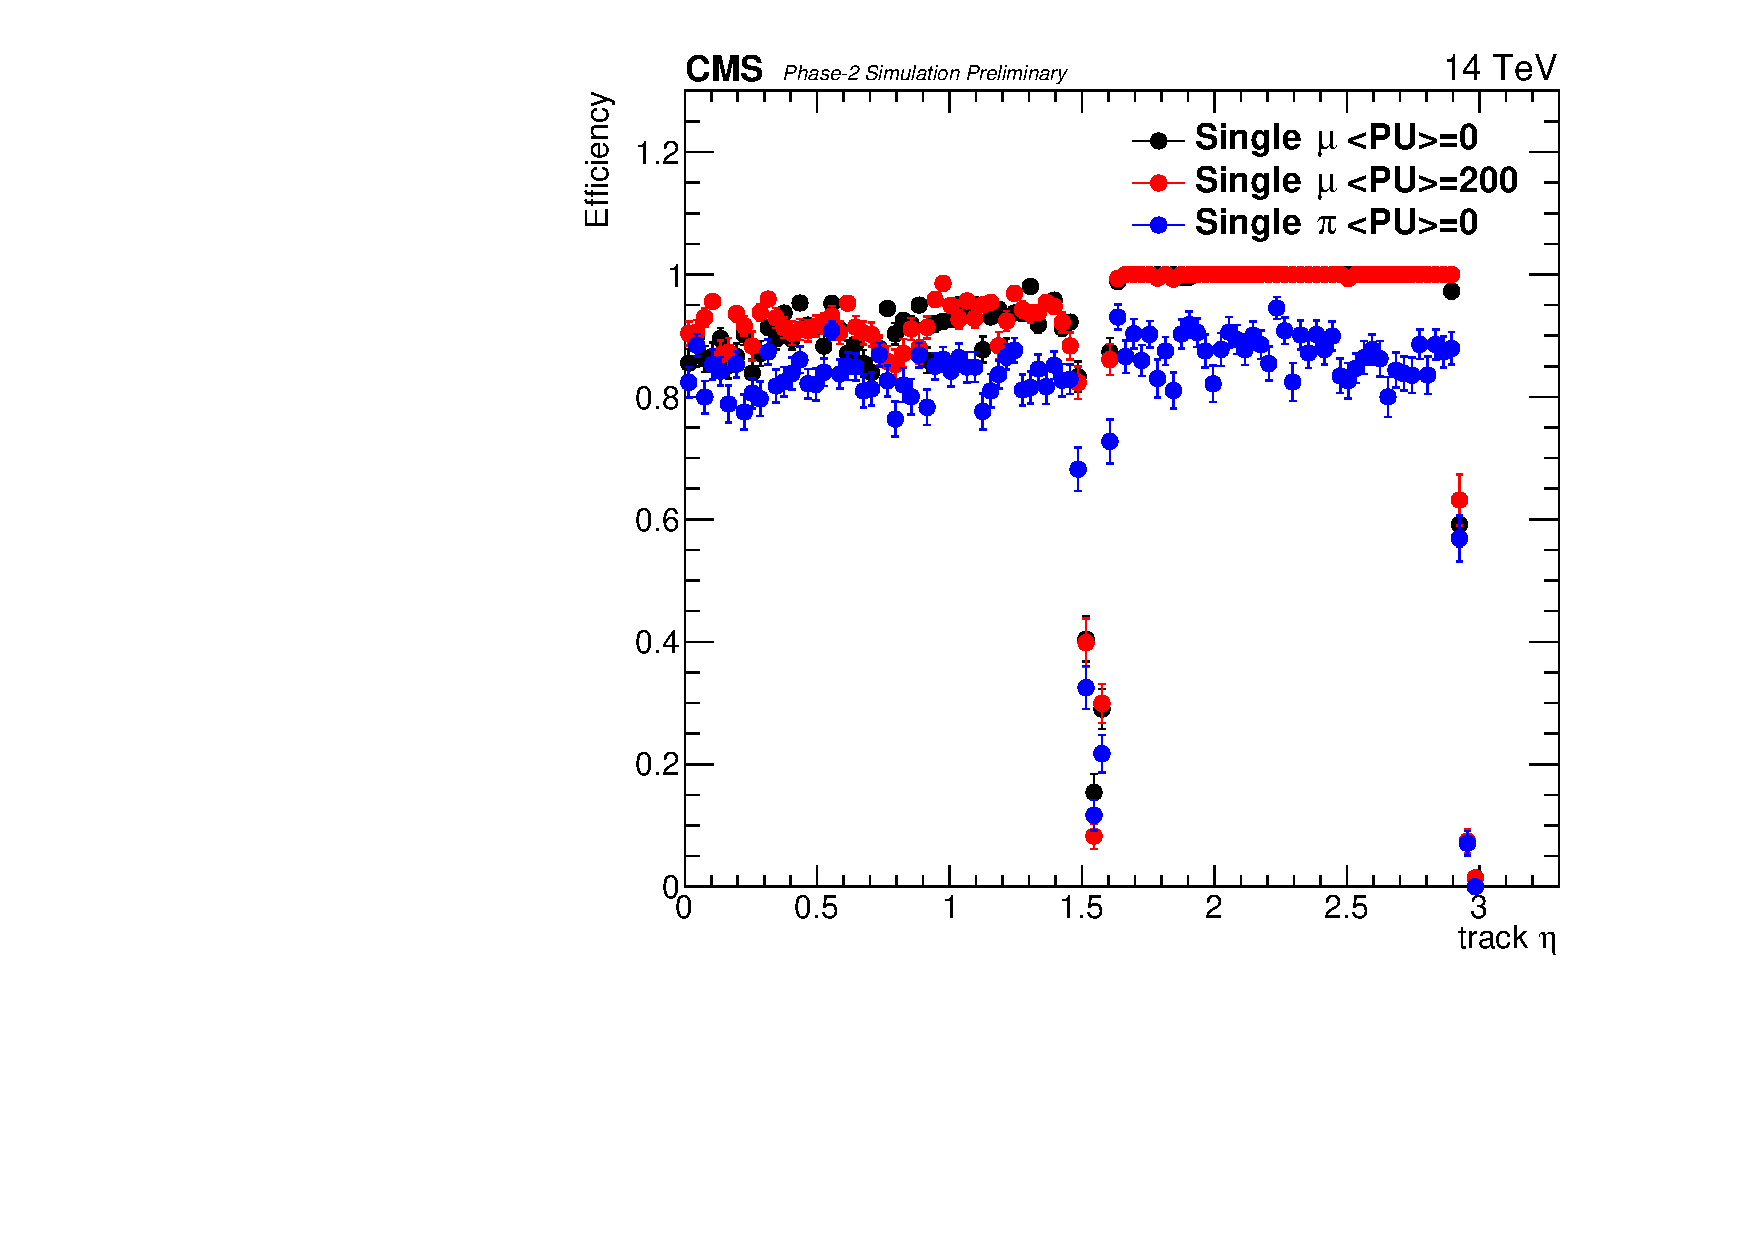
\includegraphics[width=0.48\textwidth]{fig/performance/ClusterAndTracks/divide_mtdTrack_eta_by_track_eta_mupiPUcomp.pdf}
\caption{Per-track efficiency to find an associated MTD cluster to a reconstructed track as a function of transverse momentum (left) and pseudo-rapidity (right). Tracks are matched to a generated particle in the event. Simulated particle gun events with a flat $p_T$ spectrum in the 0.7-10\mathrm{GeV} range are used. Muons (black and red dots are for events without pile-up and with average 200 pile-up events respectively) and pions (blue dots) are compared.}
\label{fig:trackclusterefficiency}
\end{figure}

The resulting time associated to the track and back-propagated to the beamline is compared to the simulation truth in Fig.~\ref{fig:trackt0vsgen}, using pions generated in simulated $t\bar{t}$ events at 14~\mathrm{TeV}. Tracks covering the BTL ($|\eta|<1.5$) and ETL ($1.5<|\eta|<3$) acceptance region are shown separately. From a fit to the distributions, the inferred time resolutions are 33~\mathrm{ps} and 35~\mathrm{ps} respectively for BTL and ETL, matching the expected simulated hit time resolutions. This also shows as expected that the track path-length estimation brings a negligible contribution to the time resolution.

\begin{figure}[!hbtp]
\centering
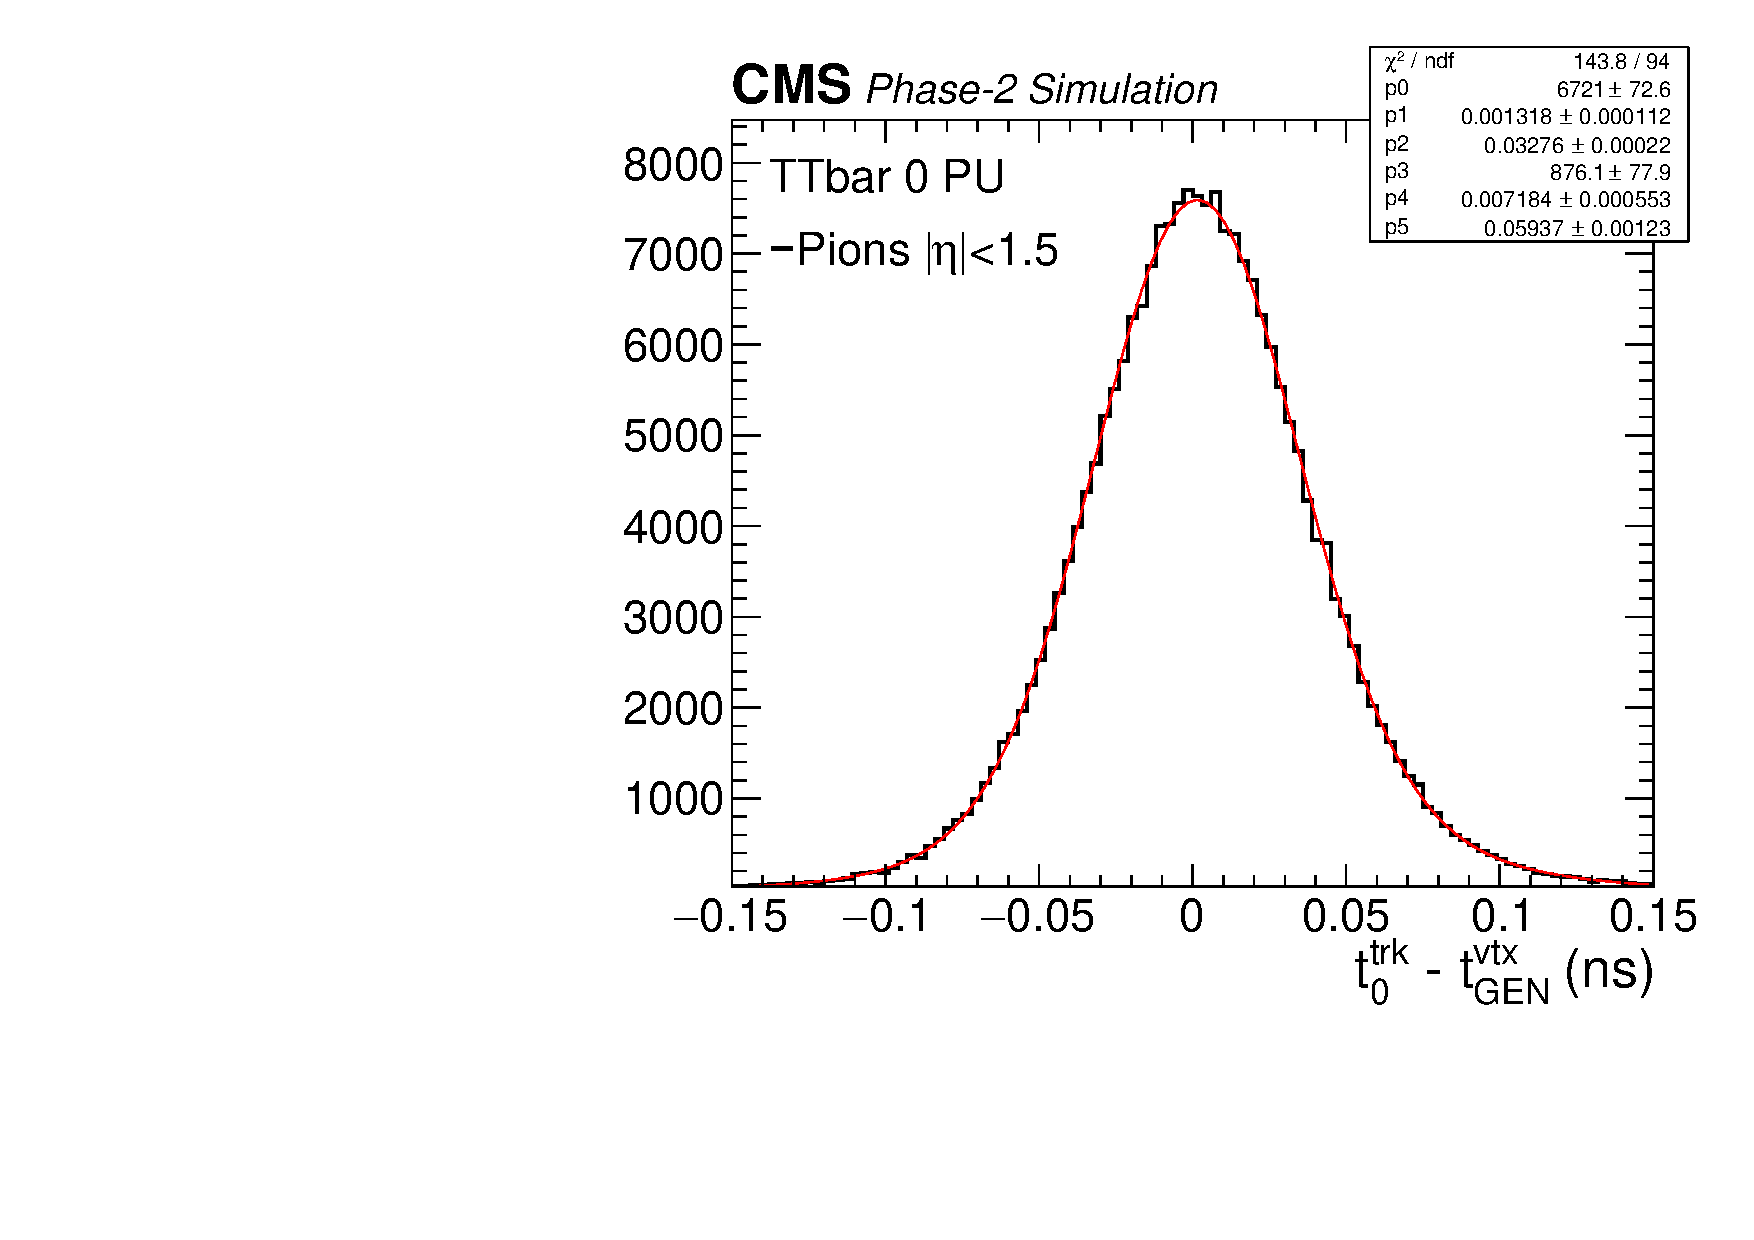
\includegraphics[width=0.48\textwidth]{fig/performance/ClusterAndTracks/res_t_pion_BTL.pdf}
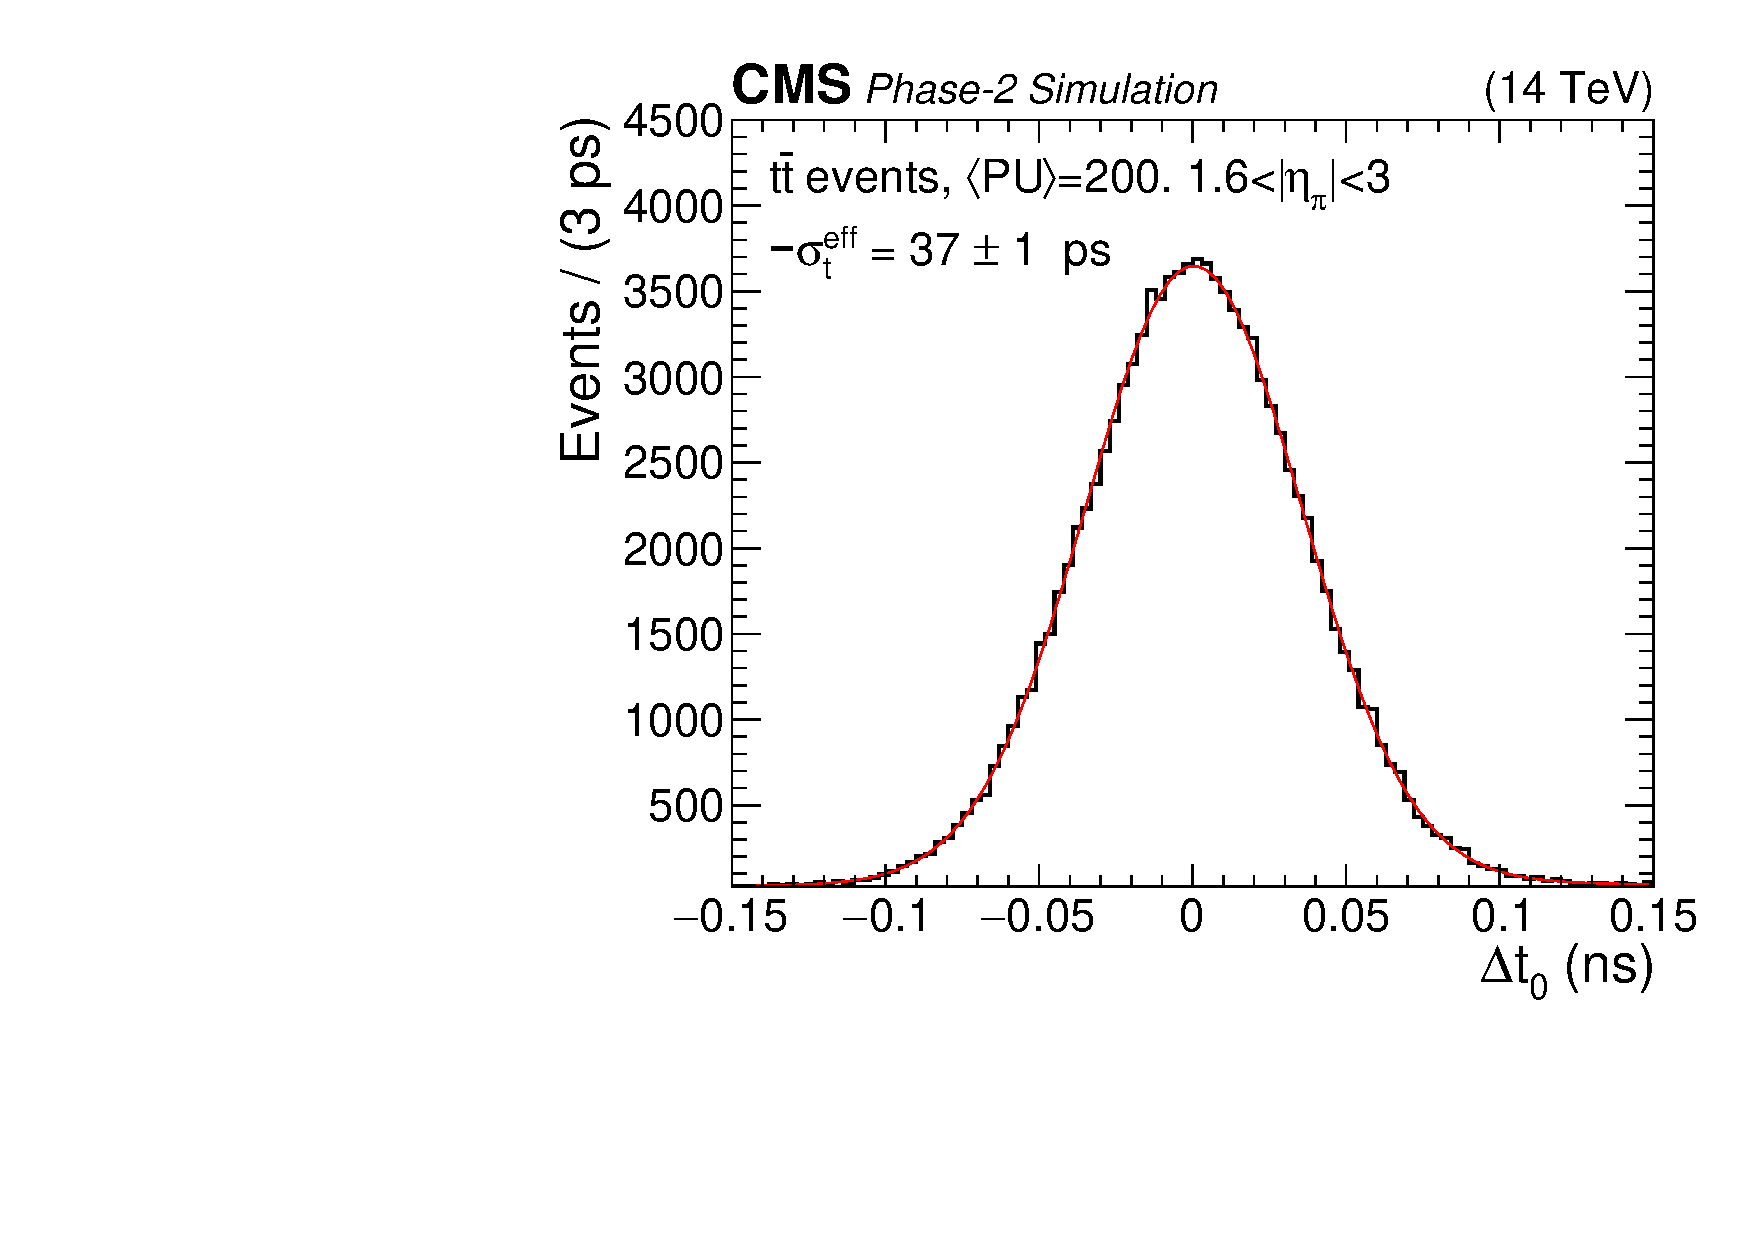
\includegraphics[width=0.48\textwidth]{fig/performance/ClusterAndTracks/res_t_pion_ETL.pdf}
\caption{Reconstructed track time at vertex respect to the simulation truth. Pions generated in simulated $t\bar{t}$ events at 14~\mathrm{TeV} are used. BTL (left) and ETL (right) acceptance regions are shown separately.}
\label{fig:trackt0vsgen}
\end{figure}
